
%(BEGIN_QUESTION)
% Copyright 2009, Tony R. Kuphaldt, released under the Creative Commons Attribution License (v 1.0)
% This means you may do almost anything with this work of mine, so long as you give me proper credit

This pH control system adds either acid or caustic to the mixing tank (but never both at the same time!) to maintain a constant pH of the water.  Recall that the addition of acid decreases the pH value of the water while the addition of caustic increases it.  The pH analytical transmitter outputs 4 mA at a pH value of 4 pH and 20 mA at a pH value of 10 pH.
 
$$\includegraphics[width=15.5cm]{i03782x01.eps}$$

Assuming direct action in the controller, determine the proper split ranges of the two control valves:

% No blank lines allowed between lines of an \halign structure!
% I use comments (%) instead, so that TeX doesn't choke.

$$\vbox{\offinterlineskip
\halign{\strut
\vrule \quad\hfil # \ \hfil & 
\vrule \quad\hfil # \ \hfil \vrule \cr
\noalign{\hrule}
%
% First row
Acid valve position & Controller output signal \cr
%
\noalign{\hrule}
%
% Another row
Fully shut (0\%) & ??? mA \cr
%
\noalign{\hrule}
%
% Another row
Wide open (100\%) & ??? mA \cr
%
\noalign{\hrule}
} % End of \halign 
}$$ % End of \vbox

% No blank lines allowed between lines of an \halign structure!
% I use comments (%) instead, so that TeX doesn't choke.

$$\vbox{\offinterlineskip
\halign{\strut
\vrule \quad\hfil # \ \hfil & 
\vrule \quad\hfil # \ \hfil \vrule \cr
\noalign{\hrule}
%
% First row
Caustic valve position & Controller output signal \cr
%
\noalign{\hrule}
%
% Another row
Fully shut (0\%) & ??? mA \cr
%
\noalign{\hrule}
%
% Another row
Wide open (100\%) & ??? mA \cr
%
\noalign{\hrule}
} % End of \halign 
}$$ % End of \vbox

\vskip 20pt \vbox{\hrule \hbox{\strut \vrule{} {\bf Suggestions for Socratic discussion} \vrule} \hrule}

\begin{itemize}
\item{} Do you suspect this process will be self-regulating, integrating, or runaway?  Explain your answer.
\item{} Do you suspect this process will have substantial lag time?  Explain your answer.
\item{} Do you suspect this process will have multiple lags?  Explain your answer.
\item{} Do you suspect this process will have substantial dead time?  Explain your answer.
\item{} What exactly is {\it pH}, and why do we care about controlling this variable in wastewater?
\item{} How is pH most commonly measured?
\item{} Identify the consequence of losing instrument air to the control valves -- what will happen to the effluent pH?
\end{itemize}

\underbar{file i03782}
%(END_QUESTION)





%(BEGIN_ANSWER)

Hint: I suggest a ``thought experiment'' whereby you imagine a process condition far from setpoint, and then you imagine what valve positions would be necessary to bring the process variable back to setpoint.

%(END_ANSWER)





%(BEGIN_NOTES)

% No blank lines allowed between lines of an \halign structure!
% I use comments (%) instead, so that TeX doesn't choke.

$$\vbox{\offinterlineskip
\halign{\strut
\vrule \quad\hfil # \ \hfil & 
\vrule \quad\hfil # \ \hfil \vrule \cr
\noalign{\hrule}
%
% First row
Acid valve position & Controller output signal \cr
%
\noalign{\hrule}
%
% Another row
Fully shut (0\%) & 12 mA \cr
%
\noalign{\hrule}
%
% Another row
Wide open (100\%) & 20 mA \cr
%
\noalign{\hrule}
} % End of \halign 
}$$ % End of \vbox

% No blank lines allowed between lines of an \halign structure!
% I use comments (%) instead, so that TeX doesn't choke.

$$\vbox{\offinterlineskip
\halign{\strut
\vrule \quad\hfil # \ \hfil & 
\vrule \quad\hfil # \ \hfil \vrule \cr
\noalign{\hrule}
%
% First row
Caustic valve position & Controller output signal \cr
%
\noalign{\hrule}
%
% Another row
Fully shut (0\%) & 12 mA \cr
%
\noalign{\hrule}
%
% Another row
Wide open (100\%) & 4 mA \cr
%
\noalign{\hrule}
} % End of \halign 
}$$ % End of \vbox

$$\includegraphics[width=15.5cm]{i03782x02.eps}$$


%INDEX% Final Control Elements, valve: split ranging
%INDEX% Process: water pH neutralization (generic)

%(END_NOTES)


